\chapter{Instantiating Nux}


\section{Design parameters}
The top-level module \code{Pu_v2} offers a large number of parameters that control various aspects of the design.
Additionally some important parameters are hidden deeper in the code.
This section lists and describes those parameters.

\subsection{Top-level parameters}
\label{sec:topopt}

First, the top-level design parameters (see also file \file{rtl/processor/pu.sv}):
\begin{description}
    \ppuParameter{OPT_BCACHE}{int}{0}{%
        Configures the branch predictor (branch cache).
        A value of 0 disables branch prediction completely.
        Higher values control the number of entries in the branch cache.
        The branch cache contains $2^{\text{\code{OPT_BCACHE}}}$ entries.
    }
    \ppuParameter{OPT_MULTIPLIER}{bit}{1}{%
        Set to one to include a fixed-point multiplier in the design.
    }
    \ppuParameter{OPT_DIVIDER}{bit}{1}{%
        Set to one to include a fixed-point divider in the design.
    }
    \ppuParameter{OPT_IOBUS}{bit}{1}{%
        Include an \gls{omnibus} interface for use by the external control facility (see~\cite{powerisa_206}).
        The interface is called \code{iobus}.
    }
    \ppuParameter{OPT_VECTOR}{bit}{1}{%
        Set to one to include the \gls{fxv} \gls{simd} extension.
        Enables also the \code{vector_bus} interface for serial load/store accesses (\code{fxvlax}, \code{fxvstax}) and \code{vector_pbus} for parallel load/store accesses (\code{fxvinx}, \code{fxvoutx}).
    }
    \ppuParameter{OPT_VECTOR_SLICES}{int}{8}{%
        Control the number of parallel datapath blocks called slices in the \gls{fxv} unit.
    }
    \ppuParameter{OPT_VECTOR_NUM_HALFWORDS}{int}{8}{%
        Control the width of the datapath of one \gls{fxv} slice in units of halfwords (\unit[16]{bit}).
        With the default configuration the unit operates on $8\times \unit[16]{bit}$ vectors.
    }
    \ppuParameter{OPT_VECTOR_MULT_DELAY}{int}{4}{%
        Configure the number of pipeline stages used for multiplication in the \gls{fxv} slices.
    }
    \ppuParameter{OPT_VECTOR_ADD_DELAY}{int}{1}{%
        Configure the number of pipeline stages used for addition in the \gls{fxv} slices.
    }
    \ppuParameter{OPT_VECTOR_INST_QUEUE_DEPTH}{int}{4}{%
        Configure the depth of the \gls{fifo} for instructions from the general-purpose part to the \gls{fxv} unit.
    }
    \ppuParameter{OPT_NEVER}{bit}{0}{%
        \textbf{Deprecated}

        Enables the \gls{never} unit for accelerated plasticity processing in \gls{hicann}.
    }
    \ppuParameter{OPT_SYNAPSE}{bit}{0}{%
        \textbf{Deprecated}

        Enables the \gls{synapse} unit for accelerated plasticity processing in \gls{hicann}.
        The \gls{synapse} unit uses the \code{syn_io_a} and \code{syn_io_b} interfaces.
    }
    \ppuParameter{OPT_DMEM}{\code{Pu_types::Opt_mem}}{\code{Pu_types::MEM_BUS}}{%
        Select whether to use the tight (\code{Pu_types::MEM_TIGHT}) or bus (\code{Pu_types::MEM_BUS}) interface to connect the data memory.
        The tight memory variant uses the \code{dmem} interface, while the bus variant uses \code{dmem_bus}.
        The bus interface is a \gls{omnibus} interface that allows for variable delay of requests with multiple requests in flight simultaneously.
        The tight interface is suitable for direct connection to a memory block.
    }
    \ppuParameter{OPT_IF_LATENCY}{int}{1}{%
        Control the number of pipeline stages between instruction memory and the rest of the frontend.
        Can be useful, when the memory is physically far away but impacts branch penalty.
    }
    \ppuParameter{OPT_BCACHE_IGNORES_JUMPS}{bit}{1}{%
        Optimization parameter to remove a long timing path.
        The branch predictor does not predict for instruction locations that are targets of branches.
    }
    \ppuParameter{OPT_BUFFER_BCTRL}{bit}{0}{%
        If set, adds a buffering register stage between the branch functional unit and the address generation unit in the instruction fetcher.
        This buffer increases branch penalty by one cycle, but removes a long timing arc through the functional unit.
    }
    \ppuParameter{OPT_WRITE_THROUGH}{bit}{1}{%
        Implement a bypass for writes to general-purpose registers, i.e.\ simultaneous reads directly use the result from the functional unit.
        Decreases length of pipeline bubbles at the cost of timing.
    }
    \ppuParameter{OPT_LOOKUP_CACHE}{bit}{1}{%
        Instruction tracking uses the lookup cache mechanism described in \cite{friedmann13phd}.
        Required if $\code{OPT_DMEM} = \code{Pu_types::MEM_BUS}$ or any other variable latency instruction is implemented.
    }
\end{description}


\subsection{Internal parameters}
Now, internal parameters in \code{rtl/packages/frontend_pkg.sv}.
Generally, these require more thinking when changing then top-level options.
For example, the multiplier latency depends on the actual multiplier implementation.
For \glspl{fpga} this might be a fixed generated core.
In that case, changing the number here will affect only the scheduling logic but not the actual multiplier latency.
So change these parameters only if you know what you are doing.

\begin{description}
        \ppuParameter{mul_latency}{int}{4}{%
            Latency of the fixed-point multiplier in cycles.
            What values are possible depends on the selected implementation (e.g.\ DesignWare block or Xilinx generated core).
        }
        \ppuParameter{div_latency}{int}{31}{%
            Latency of fixed-point divide in cycles.
        }
        \ppuParameter{ls_latency}{int}{2}{%
            Latency of load/store operations when using $\code{OPT_MEM} = \code{Pu_types::MEM_TIGHT}$.
            Possible values are 2 and 3.
            In the latter case an additional pipeline stage is added to improve timing.
        }
        \ppuParameter{ls_bus_latency}{int}{3}{%
            Expected latency of variable latency load/store operations when using $ \code{OPT_MEM} = \code{Pu_types::MEM_BUS}$.
            A wrtie-back slot is scheduled at the indicated time in the result shift register.
            If it is not used, the variable latency write-back takes over.
        }
\end{description}

\section{Interfaces and ports}

The top-level module contains the following ports and interfaces:

\begin{description}
    \portItem{clk}{logic}{Clock signal}
    \portItem{reset}{logic}{Active-high Reset signal.}
    \portItem{hold}{logic}{%
        \textbf{Deprecated}

        Active-high signal to stall instruction fetch.
        Should be tied low, or you have to check if it still works in all cases.
    }
    \portItem{imem}{Ram_if}{%
        Interface to either instruction cache or directly to memory.
        Honors the delay signal in the interface.
    }
    \portItem{dmem}{Ram_if}{%
        Interface to data memory when $ \code{OPT_MEM} = \code{Pu_types::MEM_TIGHT}$.
        Otherwise, connect dummy interface instance.
    }
    \portItem{dmem_bus}{Bus_if}{%
        \gls{omnibus} interface to data memory when $ \code{OPT_MEM} = \code{Pu_types::MEM_BUS}$.
        Otherwise, connect dummy interface instance.
    }
    \portItem{iobus}{Bus_if}{%
        \gls{omnibus} interface for the device control facility.
        Only used when \code{OPT_IOBUS} is set.
        The device control facility provides a separate address space for \gls{io}.
    }
    \portItem{vector_bus}{Bus_if}{%
        Bus for the serial load/store unit of the \gls{fxv} unit.
        Only used when \code{OPT_VECTOR} is set.
    }
    \portItem{vector_pbus}{Bus_if}{%
        Bus for the parallel load/store unit of the \gls{fxv} unit.
        Only used when \code{OPT_VECTOR} is set.
    }
    \portItem{gout}{logic[31:0]}{%
        Register mapped output for the processor.
        Is set by writing an \gls{spr}.
        Typically used for digital chip pins.
    }
    \portItem{gin}{logic[31:0]}{%
        Register mapped input for the processor.
        Is read by reading an \gls{spr}.
        Typically used for digital chip pins.
    }
    \portItem{goe}{logic[31:0]}{%
        Register mapped output enable for the processor.
        Is set by writing an \gls{spr}.
        Typically used for digital chip pins.
    }
    \portItem{ctrl}{Pu_ctrl_if}{%
        Control interface for interrupt handling, sleeping, and monitoring of program execution.
    }
    \portItem{timer}{Timer_if}{%
        Access to timer facilities.
        The timer is outside of the processor core, because it is active in sleep states during which the core's clock might be turned off.
        The timer facility also provides interrupts to the core that can trigger wake-up from the sleep state.
    }
    \portItem{syn_io_a, syn_io_b}{Syn_io_if}{%
        \textbf{Deprecated}

        \Gls{io} interfaces for \gls{synapse} unit.
    }
\end{description}


\section{Example: core environment}

\begin{figure}
    \begin{center}
        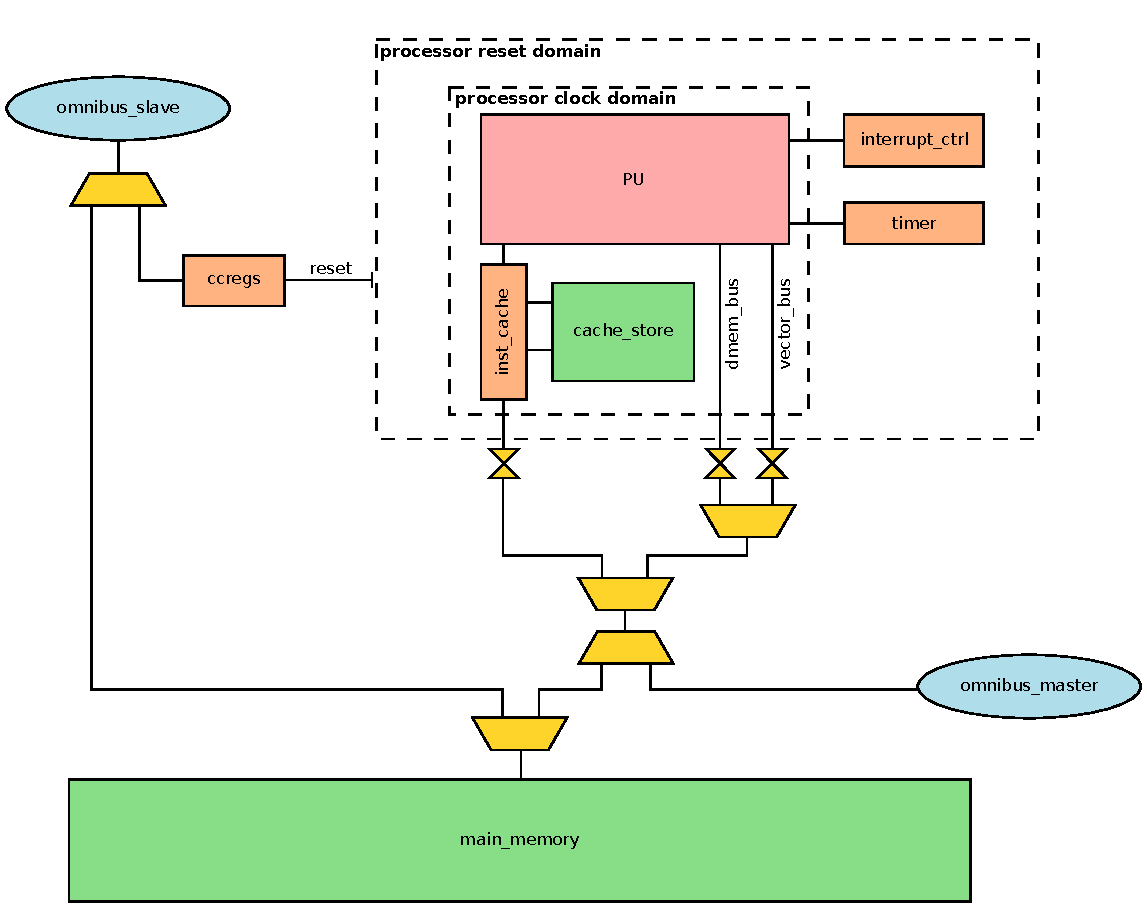
\includegraphics[width=\textwidth]{figures/ppu.pdf}
    \end{center}
    \caption[PPU instantiation example with environment]{%
        Example of environment for Nux as \gls{ppu}.
        The top-level module \code{Pu_v2} is shown as the red block labeled PU.
        The shown configuration uses a shared main memory with instruction cache.
        Data memory, instruction cache, and \gls{fxv} serial load/store all share access to the single main memory block.
        The yellow symbols represent \gls{omnibus} modules.
        A slave port allows access from the outside to change control registers (reset, clock gating) and to main memory (program loading, result retrieval).
        A master port allows access from within the \gls{ppu} to an external bus.
        The \code{interrupt_ctrl} and \code{timer} units implement interrupts and timing.
        They exist outside the clock domain controlled by control registers, but within the reset domain.
    }
    \label{fig:ppuinst}
\end{figure}

Figure~\ref{fig:ppuinst} shows an example of a simple core environment using a shared main memory.
